\chapter{Конструкторская часть}

    В данном разделе представлены схемы рассматриваемых алгоримтов и их оценка по памяти.
    
    \section{Схемы алгоритмов}
    
        \begin{figure}
            \centering
            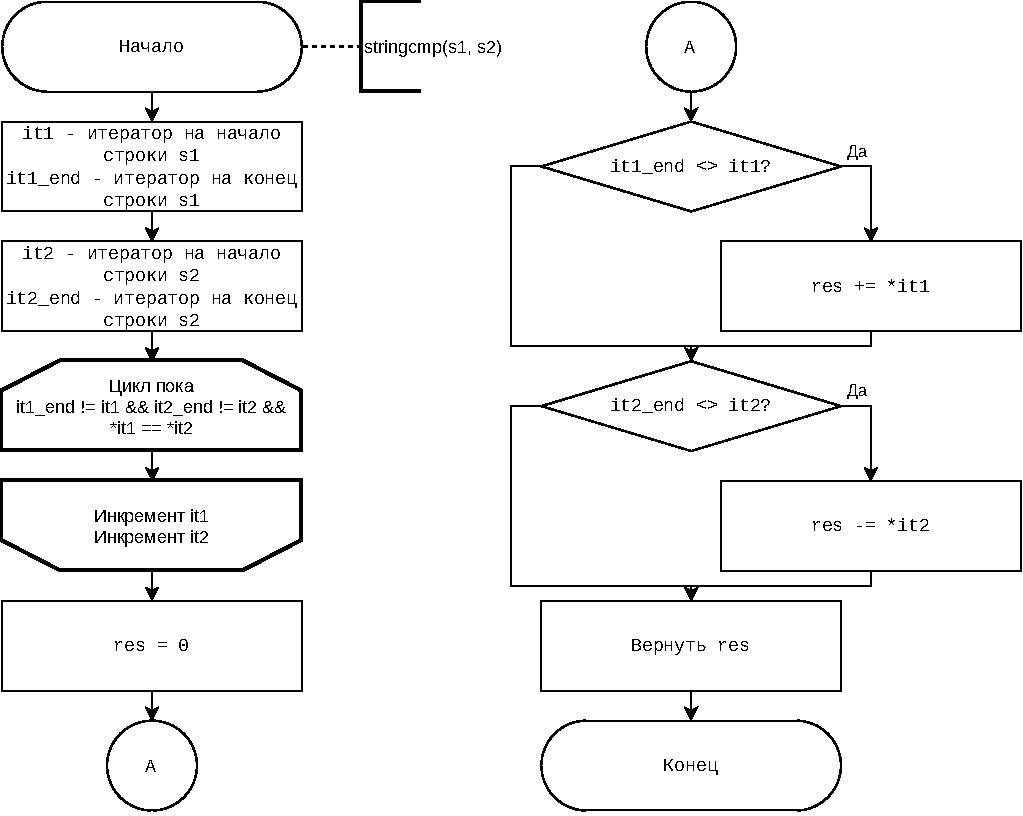
\includegraphics[width=15cm,height=25cm,keepaspectratio]{images/nonparallel.pdf}
            \caption{Последовательный алгоритм лексикографического сравнения строк}
            \label{fig:nonparallel}
        \end{figure}
        
        \begin{figure}
            \centering
            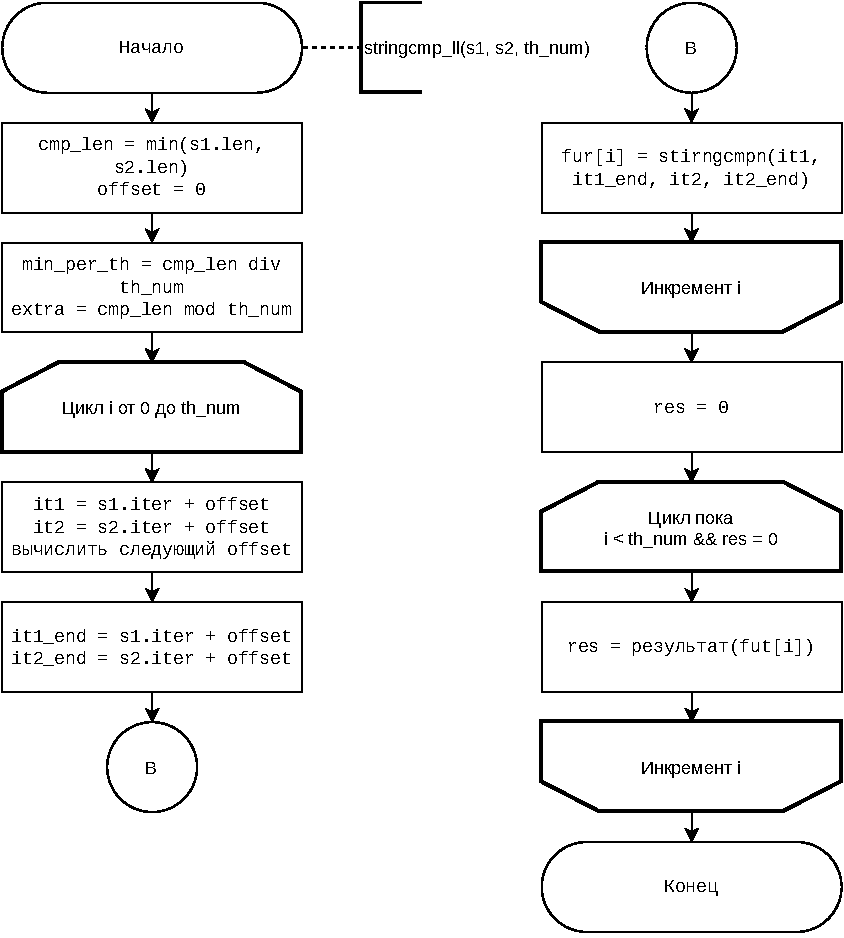
\includegraphics[width=15cm,height=25cm,keepaspectratio]{images/parallel.pdf}
            \caption{Параллельный алгоритм лексикографического сравнения строк}
            \label{fig:parallel}
        \end{figure}
        
        \begin{figure}
            \centering
            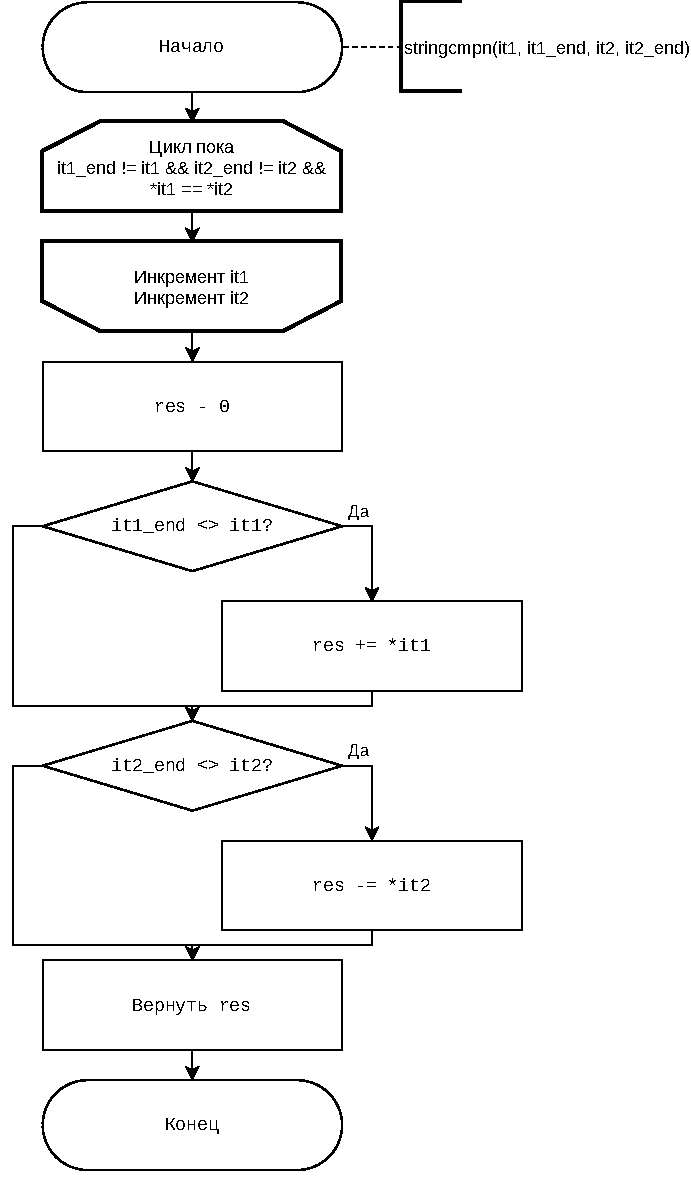
\includegraphics[width=15cm,height=22cm,keepaspectratio]{images/parallel_sub.pdf}
            \caption{Вспомогательная функция для параллельного алгоритма лексикографического сравнения строк}
            \label{fig:parallel_sub}
        \end{figure}
        
        
        \newpage
    
    \section{Структуры данных}
    
        В качестве входных данных алгоритмы принимают 2 строки, по которым рассчитывается искомое расстояние. Выходными данными алгоритма является число. Если число равно нулю, то строки равны, если число больше нуля, то первая строка больше второй иначе вторая строка больше первой.
        
        В качестве строк для реализации алгоритма выберем нуль-терминировнаныее строки. Никаких других структур данных не потребуется.
        
    \section*{Вывод}
    \addcontentsline{toc}{section}{Вывод}
    
        На основе теоретических данных, полученных из аналитического раздела были построены схемы требуемых алгоритмов.